\documentclass[11pt]{amsart}
%\pagestyle{empty} 
\setlength{\topmargin}{-0.75in} % usually -0.25in
\addtolength{\textheight}{1.25in} % usually 1.25in
\addtolength{\oddsidemargin}{-1.2in}
\addtolength{\evensidemargin}{-1.2in}
\addtolength{\textwidth}{1.9in} %\setlength{\parindent}{0pt}

\newcommand{\normalspacing}{\renewcommand{\baselinestretch}{1.1}\tiny\normalsize}
\normalspacing

% macros
\usepackage{amssymb,xspace,alltt,verbatim}
\usepackage[final]{graphicx}
\usepackage[pdftex,colorlinks=true]{hyperref}
\usepackage{fancyvrb}
\usepackage{tikz}

\newtheorem*{lem*}{Lemma}

\newcommand{\bb}{\mathbf{b}}
\newcommand{\bc}{\mathbf{c}}
\newcommand{\bs}{\mathbf{s}}
\newcommand{\bu}{\mathbf{u}}
\newcommand{\bv}{\mathbf{v}}
\newcommand{\bw}{\mathbf{w}}
\newcommand{\bx}{\mathbf{x}}
\newcommand{\by}{\mathbf{y}}

\newcommand{\bbf}{\mathbf{f}}

\newcommand{\CC}{{\mathbb{C}}}
\newcommand{\RR}{{\mathbb{R}}}
\newcommand{\eps}{\epsilon}
\newcommand{\ZZ}{{\mathbb{Z}}}
\newcommand{\ZZn}{{\mathbb{Z}}_n}
\newcommand{\NN}{{\mathbb{N}}}
\newcommand{\ip}[2]{\mathrm{\left<#1,#2\right>}}

\renewcommand{\Re}{\operatorname{Re}}
\renewcommand{\Im}{\operatorname{Im}}

\newcommand{\Log}{\operatorname{Log}}

\newcommand{\grad}{\nabla}

\newcommand{\ds}{\displaystyle}

\newcommand{\Matlab}{\textsc{Matlab}\xspace}
\newcommand{\Octave}{\textsc{Octave}\xspace}
\newcommand{\pylab}{\textsc{pylab}\xspace}

\newcommand{\prob}[1]{\bigskip\noindent\textbf{#1.} }
\newcommand{\cprob}[1]{\bigskip\noindent\underline{\textbf{#1.}} }
\newcommand{\pts}[1]{(\emph{#1 pts})}

\newcommand{\probpts}[2]{\prob{#1} \pts{#2} \quad}
\newcommand{\cprobpts}[2]{\cprob{#1} \pts{#2} \quad}
\newcommand{\ppartpts}[2]{\textbf{(#1)} \pts{#2} \quad}
\newcommand{\epartpts}[2]{\medskip\noindent \textbf{(#1)} \pts{#2} \quad}


\begin{document}
\hfill \Large Name:\underline{\phantom{Ed Bueler really really long long long name}}
\medskip

\scriptsize \noindent Math 252 Calculus 2 (Bueler) \hfill Tuesday, 13 December 2022 %Tuesday, 13 December 2022
\medskip

\LARGE\centerline{\textbf{Final Exam}}

\smallskip
\begin{quote}
\large
\textbf{No book, electronics, calculator, or internet access.  125 points possible.  125 minutes maximum.  Allowed notes: 1/2 sheet of letter paper (i.e.~half of $8.5\times 11$ sheet), with anything written on both sides.}
\end{quote}

\normalsize
\medskip

\thispagestyle{empty}

\prob{1}  \ppartpts{a}{5} Sketch the region bounded by $\displaystyle y=\frac{1}{x}$ and the $x$-axis, on the interval $1 \le x < +\infty$.
\vfill

\epartpts{b}{8} Compute the volume of the solid of revolution found by rotating the region in \textbf{(a)} around the $x$-axis, or show that it is infinite.
\vfill

\clearpage\newpage
\probpts{2}{7}  Set up, but \textbf{do not evaluate}, an integral for the arclength of the parametric curve defined by $\displaystyle x(t) = e^t$, $y(t) = \ln t$ on the interval $1\leq t\le 10$.
\vfill

\probpts{3}{8}  Compute the indefinite integral:
\large
    $$\int x \,5^{x^2}\,dx = \hspace{5.0in}$$
\normalsize
\vfill


\clearpage\newpage
\prob{4}  Evaluate the integrals:

\epartpts{a}{6} $\ds  \int_0^3 x\, e^{-x}\,dx =$
\vfill

\epartpts{b}{6} $\ds  \int \frac{dx}{x(1+x)} =$
\vfill

\clearpage\newpage
\prob{5}  Evaluate the indefinite integrals:

\epartpts{a}{6} $\ds  \int \cos^2 \theta \sin^2\theta\,d\theta =$
\vfill

\epartpts{b}{6} $\ds  \int \frac{dz}{\sqrt{1+z^2}} =$
\vfill


\clearpage\newpage
\prob{6}  Determine whether the following series converge or diverge. Explain your reasoning and identify any test used.

\epartpts{a}{6}  $\ds \sum_{n = 0}^\infty \frac{(-1)^n}{\sqrt{n+3}}$
\vfill

\epartpts{b}{6}  $\ds \sum_{n = 1}^\infty \frac{n}{10 + \sqrt{n}}$
\vfill


\clearpage\newpage
\prob{7}  \ppartpts{a}{8}  Find the Maclaurin series by any convenient method:
\large
    $$f(x) = x^2 e^{-x^2} \hspace{5.0in}$$
\normalsize
\vfill

\epartpts{b}{8}  Use the result in \textbf{(a)} to compute the following antiderivative as a power series:
\large
    $$\int x^2 e^{-x^2}\,dx = \hspace{5.0in}$$
\normalsize
\vfill


\clearpage\newpage
\prob{8}  \ppartpts{a}{6}  Does the series $\ds \sum_{n=1}^\infty \frac{n}{2^n}$ converge or diverge?  Explain your reasoning and identify any test used.
\vspace{2.5in}

\epartpts{b}{5}  Compute and simplify $S_3$ for the series in part \textbf{(a)}.
\vspace{1.5in}

\probpts{9}{6}  Make a careful and reasonably-large sketch of the cardiod $r = 1 - \sin\theta$.  (\emph{Label the axes and give dimensions/values along the axes.})
\vfill


\clearpage\newpage
\prob{10}  Consider the parametric curve $\ds x = t + \frac{1}{t}$, $\ds y = t - \frac{1}{t}$.

\epartpts{a}{6}  Find the equation of the tangent line at $t=1$.
\vfill

\epartpts{b}{6}  Compute the second derivative $\ds \frac{d^2 y}{dx^2}$.
\vfill


\clearpage\newpage
\probpts{11}{8}  Find the radius and interval of convergence of the power series:
    $$\sum_{n = 1}^\infty \frac{(x + 5)^n}{n^2} \hspace{5.0in}$$
\vfill

\probpts{12}{8}  Find the general solution to the differential equation $y' = \ln x + \tan x$.
\vfill


\clearpage\newpage
\probpts{Extra Credit}{3}  First, explain in terms of familiar Maclaurin series, why $\ds \frac{1}{e} = \sum_{n=0}^\infty \frac{(-1)^n}{n!}$.  Second, how accurate is $\ds S_{9} = \sum_{n=0}^{9} \frac{(-1)^n}{n!}$ as an approximation to $1/e$?  Write your bound on the error in the box below.

\vfill
\hspace{-4mm} $\ds |R_{9}| = \left|S_{9} - \frac{1}{e}\right| \le \boxed{\phantom{\begin{matrix} lakjsd alsfjd \\ sdfa \\ sdaf \end{matrix}}}$
\bigskip

\noindent \hrule
\small
\bigskip
\noindent You may find the following \textbf{trigonometric formulas} useful.  However, there are other trig.~formulas, not listed here, which you should have in memory, or which can be derived from these.

\begin{align*}
\sin(\alpha \pm \beta) &= \sin \alpha \cos \beta \pm \cos \alpha \sin \beta \\
\cos(\alpha \pm \beta) &= \cos \alpha \cos \beta \mp \sin \alpha \sin \beta \\
\sin(ax) \sin(bx) &= \frac{1}{2} \cos((a-b)x) - \frac{1}{2} \cos((a+b)x) \\
\sin(ax) \cos(bx) &= \frac{1}{2} \sin((a-b)x) + \frac{1}{2} \sin((a+b)x) \\
\cos(ax) \cos(bx) &= \frac{1}{2} \cos((a-b)x) + \frac{1}{2} \cos((a+b)x)
\end{align*}

\bigskip
\noindent \hrule
\small
\medskip
\centerline{\footnotesize \textsc{extra space for answers}}
\vspace{2.5in}


\clearpage\newpage
\large\centerline{\textbf{Summary of Convergence Tests}}
\normalsize

\begin{center}
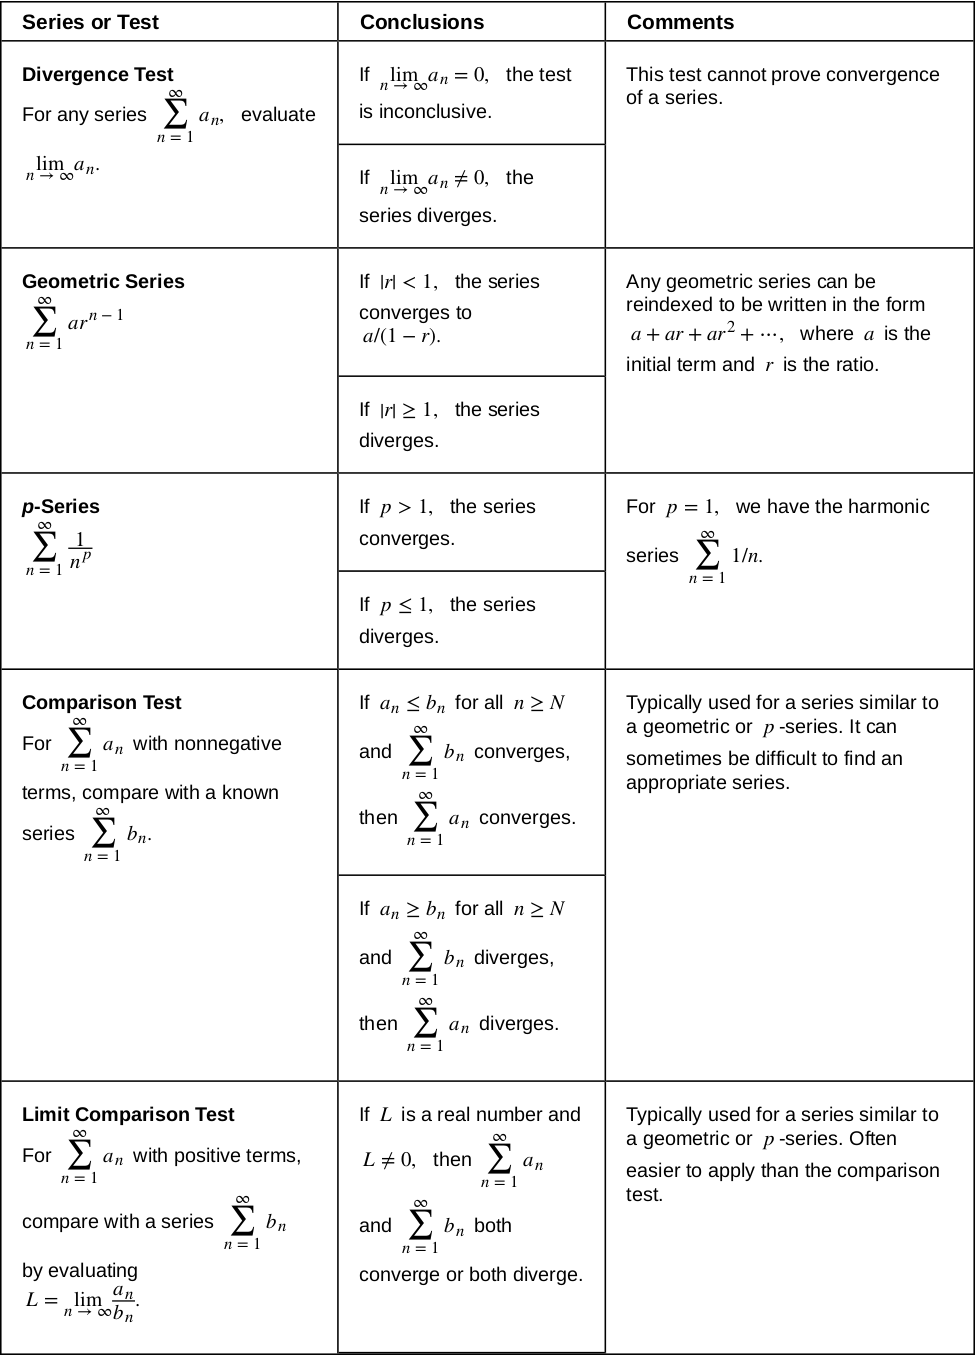
\includegraphics[width=0.95\textwidth]{figs/serieshandoutA.png}
\end{center}
\vfill


\clearpage\newpage
\begin{center}
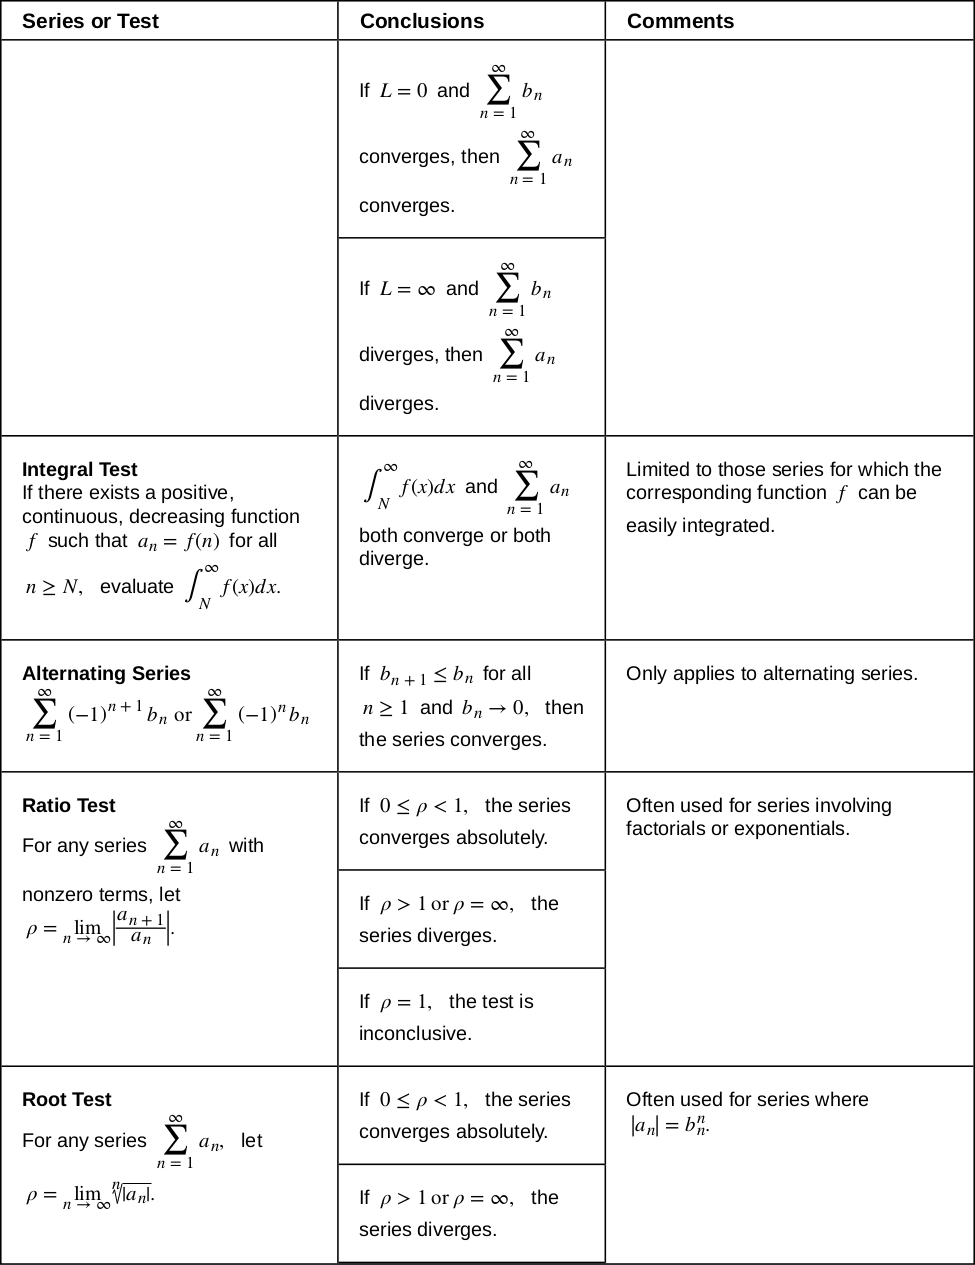
\includegraphics[width=0.95\textwidth]{figs/serieshandoutB.png}

\vspace{-2mm}

\includegraphics[width=0.95\textwidth]{figs/serieshandoutC.png}
\end{center}
\vfill

\end{document}
